\documentclass{article}\usepackage[]{graphicx}\usepackage[]{color}
%% maxwidth is the original width if it is less than linewidth
%% otherwise use linewidth (to make sure the graphics do not exceed the margin)
\makeatletter
\def\maxwidth{ %
  \ifdim\Gin@nat@width>\linewidth
    \linewidth
  \else
    \Gin@nat@width
  \fi
}
\makeatother

\definecolor{fgcolor}{rgb}{0.345, 0.345, 0.345}
\newcommand{\hlnum}[1]{\textcolor[rgb]{0.686,0.059,0.569}{#1}}%
\newcommand{\hlstr}[1]{\textcolor[rgb]{0.192,0.494,0.8}{#1}}%
\newcommand{\hlcom}[1]{\textcolor[rgb]{0.678,0.584,0.686}{\textit{#1}}}%
\newcommand{\hlopt}[1]{\textcolor[rgb]{0,0,0}{#1}}%
\newcommand{\hlstd}[1]{\textcolor[rgb]{0.345,0.345,0.345}{#1}}%
\newcommand{\hlkwa}[1]{\textcolor[rgb]{0.161,0.373,0.58}{\textbf{#1}}}%
\newcommand{\hlkwb}[1]{\textcolor[rgb]{0.69,0.353,0.396}{#1}}%
\newcommand{\hlkwc}[1]{\textcolor[rgb]{0.333,0.667,0.333}{#1}}%
\newcommand{\hlkwd}[1]{\textcolor[rgb]{0.737,0.353,0.396}{\textbf{#1}}}%

\usepackage{framed}
\makeatletter
\newenvironment{kframe}{%
 \def\at@end@of@kframe{}%
 \ifinner\ifhmode%
  \def\at@end@of@kframe{\end{minipage}}%
  \begin{minipage}{\columnwidth}%
 \fi\fi%
 \def\FrameCommand##1{\hskip\@totalleftmargin \hskip-\fboxsep
 \colorbox{shadecolor}{##1}\hskip-\fboxsep
     % There is no \\@totalrightmargin, so:
     \hskip-\linewidth \hskip-\@totalleftmargin \hskip\columnwidth}%
 \MakeFramed {\advance\hsize-\width
   \@totalleftmargin\z@ \linewidth\hsize
   \@setminipage}}%
 {\par\unskip\endMakeFramed%
 \at@end@of@kframe}
\makeatother

\definecolor{shadecolor}{rgb}{.97, .97, .97}
\definecolor{messagecolor}{rgb}{0, 0, 0}
\definecolor{warningcolor}{rgb}{1, 0, 1}
\definecolor{errorcolor}{rgb}{1, 0, 0}
\newenvironment{knitrout}{}{} % an empty environment to be redefined in TeX

\usepackage{alltt}

\usepackage[titletoc]{appendix}
\usepackage{listings}
\usepackage{hyperref}
\usepackage{url}
\usepackage[backend=bibtex, sorting=none]{biblatex}


\bibliography{references}
\IfFileExists{upquote.sty}{\usepackage{upquote}}{}

\begin{document}




\title{Computational Network Analysis - Class Project \\ Wikipedia Navigation Paths}
\author{Tobias Kloht, ID: 4596192}
\maketitle
\section{Introduction}
Wikipedia defines itself as "a collaboratively edited, multilingual, free Internet encyclopedia" \cite{wiki:def} covering more than 4.4 million articles in the english language version. It is ranked 6th among the most popular websites worldwide \cite{alexa:wiki} and has developed into the de-facto standard for free user generated encyclopedic content.

This class project aims to analyze the behaviour of users browsing Wikipedia by aggregating internal links used when searching for a specific information into a network. Apart from finding common patterns and analyzing the user behaviour in general, this could potentialy reveal problems with the site's navigation and highlight possible improvements.

\section{Dataset}
The dataset used in this project contains navigation paths on Wikipedia, collected through the game Wikispeedia \cite{wikispeedia}. The idea of this game is to navigate from one given article to another, using only internal links and as few steps as possible. It was developed as part of a research project to acquire data on commonsense knowledge \cite{wikispeedia:article}. The game operates on a condensed subset of Wikipedia consisting of 4600 articles from 2007.

The resulting dataset consists of 51,318 finished navigation paths and can be accessed at the Stanford Network Analysis Project \cite{snap}. Unfinished navigation paths are also available but have not been used in this project.

\section{Adjusting the Data Format}
While the dataset described above clearly represents a network with articles as vertices and links as edges, the provided data had to be adjusted for usage with the igraph library \cite{igraph}. To illustrate this, the following listing is an excerpt of the data, provided as a tab-separated list. 

The columns from left to right are:
\begin{itemize}
\item Hashed IP Address
\item Timestamp
\item Duration in seconds
\item Path given as list of articles separated by ";"
\item Rating - optinally provided by users after finishing the game
\end{itemize}

In addition to that, back clicks are represented as "\textless".
\lstset{
  numbers=left,
  basicstyle=\ttfamily\scriptsize,
  frame=single,
  breaklines=true,
  tabsize=2
}
\begin{lstlisting}[title=Excerpt: Wipispeedia Dataset ]
36dabfa133b20e3c  1249525912	112	14th_century;China;Gunpowder;Fire	2
20418ff4797f96be	1229188046	139	14th_century;Time;Isaac_Newton;Light;Color;Rainbow	1
08888b1b428dd90e	1232241510	74	14th_century;Time;Light;Rainbow	3
\end{lstlisting}

The main problem is that this does not define a network but a list of paths clicked through by users. In order to allow processing of the data with R and igraph I have decided to transform the data into a network as follows:
\begin{description}
\item[Vertices:] The articles 
\item[Edges:] The links used to navigate between two articles
\item[Edge Weights:] The amount of times a link has been used
\end{description}

In this format the representation of back clicks is problematic, because it results in a vertex labeled "\textless" with ingoing edges for each back click. For this project it makes more sense to replace each "\textless" with the article that the back click leads to. For example, an entry of the form
\begin{lstlisting}
408362e90dc90bce  1249103594	61	Asia;Japan;Cereal;<;<;Japan;Fishing;<;Meat;Mammal	NULL
\end{lstlisting}
would be transformed to 
\begin{lstlisting}
408362e90dc90bce  1249103594  61	Asia;Japan;Cereal;Japan;Asia;Japan;Fishing;Japan;Meat;Mammal	NULL
\end{lstlisting}

\subsection{The Large Graph Layout format}
The resulting network will be stored in the Large Graph Layout (LGL) format \cite{lgl}, which is essentially a modified adjacency list. It lists each vertex preceded by a pound sign, followed by all vertices sharing an edge with it on subsequent lines. Each neighboring vertex can optionally have a weight attached to it.

\begin{lstlisting}[title=LGL format example ]
# vertex1name
vertex2name [optionalWeight]
vertex3name [optionalWeight]
\end{lstlisting}


\subsection{Conversion Steps}

The provided data was transformed to the format described above in the following steps:

\begin{enumerate}
\item Normalize navigation path by replacing "back clicks" with the actual article
\item Extract all vertices, i.e. articles
\item For each vertex, find neighboring vertices and store both in the LGL format 
\end{enumerate}

In step three the navigation paths are iterated for each article. Whenever an entry matching the current article is found, the next entry of the navigation list is added to a temporary list. After this is done for all navigation paths, the temporary list holds all neighboring articles of the current vertex and it is easy to construct the format discussed above. The other steps are straightforward and will not be discussed further.

Each step has been implemented as a Ruby script. All scripts are available in Appendix A as well as \href{https://github.com/t-obi/computational-network-analysis/tree/master/project/wikispeedia_paths-and-graph}{Github}.


\section{Analyzing the Network}
The resulting network can be imported by igraph directly. A simple plot of the network provides the following:
\begin{knitrout}
\definecolor{shadecolor}{rgb}{0.969, 0.969, 0.969}\color{fgcolor}\begin{kframe}
\begin{alltt}
\hlkwd{plot.igraph}\hlstd{(wikispeedia,} \hlkwc{vertex.size} \hlstd{=} \hlnum{2}\hlstd{,} \hlkwc{vertex.label} \hlstd{=} \hlnum{NA}\hlstd{,} \hlkwc{edge.arrow.width} \hlstd{=} \hlnum{0.02}\hlstd{,}
    \hlkwc{edge.arrow.size} \hlstd{=} \hlnum{0.2}\hlstd{,} \hlkwc{edge.width} \hlstd{=} \hlnum{0.2}\hlstd{,} \hlkwc{layout} \hlstd{= layout.kamada.kawai)}
\end{alltt}
\end{kframe}
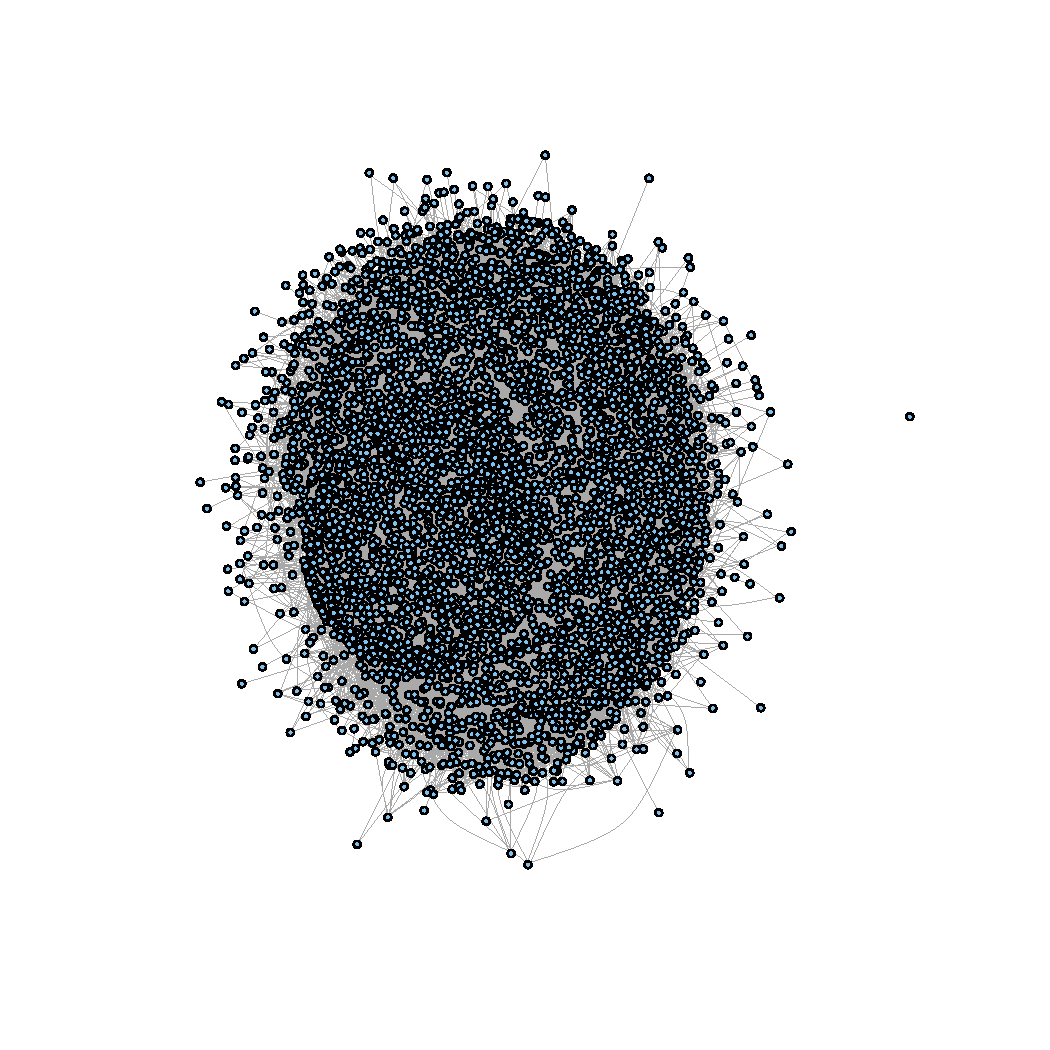
\includegraphics[width=\maxwidth]{figure/unnamed-chunk-1} 

\end{knitrout}



To get an initial overview the size of the network can be examined:
\begin{knitrout}
\definecolor{shadecolor}{rgb}{0.969, 0.969, 0.969}\color{fgcolor}\begin{kframe}
\begin{alltt}
\hlcom{# number of vertices}
\hlkwd{vcount}\hlstd{(wikispeedia)}
\end{alltt}
\begin{verbatim}
## [1] 4170
\end{verbatim}
\begin{alltt}
\hlcom{# number of edges}
\hlkwd{ecount}\hlstd{(wikispeedia)}
\end{alltt}
\begin{verbatim}
## [1] 59530
\end{verbatim}
\end{kframe}
\end{knitrout}


\subsection{Degree Distribution}
The next step will be a look at the degrees and their distribution:

\begin{knitrout}
\definecolor{shadecolor}{rgb}{0.969, 0.969, 0.969}\color{fgcolor}\begin{kframe}
\begin{alltt}
\hlcom{# mean degree of the network}
\hlkwd{mean}\hlstd{(}\hlkwd{degree}\hlstd{(wikispeedia))}
\end{alltt}
\begin{verbatim}
## [1] 28.55
\end{verbatim}
\begin{alltt}
\hlcom{# median degree of the network}
\hlkwd{median}\hlstd{(}\hlkwd{degree}\hlstd{(wikispeedia))}
\end{alltt}
\begin{verbatim}
## [1] 14
\end{verbatim}
\begin{alltt}
\hlcom{# max degree of the network}
\hlkwd{max}\hlstd{(}\hlkwd{degree}\hlstd{(wikispeedia))}
\end{alltt}
\begin{verbatim}
## [1] 1639
\end{verbatim}
\end{kframe}
\end{knitrout}


This shows that the networks degree is right-skewed, i.e. the mean degree is significantly larger than the median. This is a first hint that a small number of vertices has significantly more edges than the rest of the network. To investigate this further we will calculate the degree centralization. 
\begin{knitrout}
\definecolor{shadecolor}{rgb}{0.969, 0.969, 0.969}\color{fgcolor}\begin{kframe}
\begin{alltt}
\hlkwd{centralization.degree}\hlstd{(wikispeedia)}\hlopt{$}\hlstd{centralization}
\end{alltt}
\begin{verbatim}
## [1] 0.3863
\end{verbatim}
\end{kframe}
\end{knitrout}

This result is relatively high and supports our assumption above. The degree centrality is distributed as follows:

\begin{knitrout}
\definecolor{shadecolor}{rgb}{0.969, 0.969, 0.969}\color{fgcolor}\begin{kframe}
\begin{alltt}
\hlkwd{plot}\hlstd{(}\hlkwd{centralization.degree}\hlstd{(wikispeedia)}\hlopt{$}\hlstd{res,} \hlkwc{type} \hlstd{=} \hlstr{"l"}\hlstd{)}
\end{alltt}
\end{kframe}
\includegraphics[width=\maxwidth]{figure/degree_centrality_plot} 
\begin{kframe}\begin{alltt}
\hlcom{# mean degree}
\hlkwd{mean}\hlstd{(}\hlkwd{centralization.degree}\hlstd{(wikispeedia)}\hlopt{$}\hlstd{res)}
\end{alltt}
\begin{verbatim}
## [1] 28.55
\end{verbatim}
\begin{alltt}
\hlcom{# max degree}
\hlkwd{max}\hlstd{(}\hlkwd{centralization.degree}\hlstd{(wikispeedia)}\hlopt{$}\hlstd{res)}
\end{alltt}
\begin{verbatim}
## [1] 1639
\end{verbatim}
\end{kframe}
\end{knitrout}


This data further exemplifies that the degree is very unevenly distributed among the network, which means that a small number of articles has been \mbox{navigated} frequently in the game. One article in particular has a very high degree even in comparison to all other vertices with high degrees. To find out which article is represented by this vertex the following command can be used:
\begin{knitrout}
\definecolor{shadecolor}{rgb}{0.969, 0.969, 0.969}\color{fgcolor}\begin{kframe}
\begin{alltt}
\hlkwd{which}\hlstd{(}\hlkwd{degree}\hlstd{(wikispeedia)} \hlopt{==} \hlkwd{max}\hlstd{(}\hlkwd{degree}\hlstd{(wikispeedia)))}
\end{alltt}
\begin{verbatim}
## United_States 
##           136
\end{verbatim}
\end{kframe}
\end{knitrout}

The reason why the article about the United States of America has been used so frequently in this experiment is beyond the scope of this class project. However, given that the initial intention of the Wikispeedia project is to analyze commonsense knowledge, it could be assumed that the users of the game shared a basic understanding of that subject and used it to derive further information.

\subsection{Betweenness Distribution}
When analyzing the betweenness similar results to the degree section can be expected.

\begin{knitrout}
\definecolor{shadecolor}{rgb}{0.969, 0.969, 0.969}\color{fgcolor}\begin{kframe}
\begin{alltt}
\hlkwd{centralization.betweenness}\hlstd{(wikispeedia)}\hlopt{$}\hlstd{centralization}
\end{alltt}
\begin{verbatim}
## [1] 0.2035
\end{verbatim}
\end{kframe}
\end{knitrout}

This result is in line with our expectations and shows a relatively centralized distribution of the betweenness over the network.

\begin{knitrout}
\definecolor{shadecolor}{rgb}{0.969, 0.969, 0.969}\color{fgcolor}\begin{kframe}
\begin{alltt}
\hlkwd{plot}\hlstd{(}\hlkwd{centralization.betweenness}\hlstd{(wikispeedia)}\hlopt{$}\hlstd{res,} \hlkwc{type} \hlstd{=} \hlstr{"l"}\hlstd{)}
\end{alltt}
\end{kframe}
\includegraphics[width=\maxwidth]{figure/betweenness_centrality_plot} 
\begin{kframe}\begin{alltt}
\hlcom{# mean betweenness}
\hlkwd{mean}\hlstd{(}\hlkwd{centralization.betweenness}\hlstd{(wikispeedia)}\hlopt{$}\hlstd{res)}
\end{alltt}
\begin{verbatim}
## [1] 3632
\end{verbatim}
\begin{alltt}
\hlcom{# max betweenness}
\hlkwd{max}\hlstd{(}\hlkwd{centralization.betweenness}\hlstd{(wikispeedia)}\hlopt{$}\hlstd{res)}
\end{alltt}
\begin{verbatim}
## [1] 1771100
\end{verbatim}
\end{kframe}
\end{knitrout}


The Plot above further shows the similarity between degree and betweenness distribution in this graph. In the next step we will test if the same article shares maximum betweenness and degree:
\begin{knitrout}
\definecolor{shadecolor}{rgb}{0.969, 0.969, 0.969}\color{fgcolor}\begin{kframe}
\begin{alltt}
\hlkwd{which}\hlstd{(}\hlkwd{betweenness}\hlstd{(wikispeedia)} \hlopt{==} \hlkwd{max}\hlstd{(}\hlkwd{betweenness}\hlstd{(wikispeedia)))}
\end{alltt}
\begin{verbatim}
## United_States 
##           136
\end{verbatim}
\end{kframe}
\end{knitrout}


This expectation is true as well. In this case this just shows that the article which is used the most also interconnects the most articles, which is only natural given the premise of this experiment.

\subsection{Path Length}
The analysis to this point makes it very likely that the small-world phenomenon applies to this network. To confirm this we can calculate the average path length of the network:
\begin{knitrout}
\definecolor{shadecolor}{rgb}{0.969, 0.969, 0.969}\color{fgcolor}\begin{kframe}
\begin{alltt}
\hlkwd{average.path.length}\hlstd{(wikispeedia)}
\end{alltt}
\begin{verbatim}
## [1] 2.743
\end{verbatim}
\end{kframe}
\end{knitrout}

This shows that the articles in the network can be reached with very few hops on average.

\section{Conclusion}
To summarize, we found that the examined network shows typical characteristics of similar networks. The relatively high centralization leads to a short path length because a small set of nodes can interconnect many other vertices.

For further analysis it would be interesting to identify communities within the network, this proved difficult during this class project due to the size of the dataset. 




\newpage 
\printbibliography

\newpage 
\begin{appendices}
  \section{Scripts for Data Transformation}
  \lstinputlisting[language=Ruby,caption={Node Extraction},label=node_extraction]{wikispeedia_paths-and-graph/read_nodes.rb}
  \lstinputlisting[language=Ruby,caption={Path normalization},label=path_normalization]{wikispeedia_paths-and-graph/fix_paths.rb}
  \lstinputlisting[language=Ruby,caption={Building the Network},label=read_edges]{wikispeedia_paths-and-graph/read_edges.rb}
  
\end{appendices}
\end{document}
